\section{Modelado Matem�tico }\index{Modelado!Modelado Matem�tico}
En el modelo matem�tico se encuentran incluidos todos los factores que intervienen en el comportamiento del robot y dependiendo del tipo de modelado, se puede obtener una simulaci�n del comportamiento real del robot.\\

La cinem�tica estudia el movimiento de alg�n sistema sin tomar en cuenta las fuerzas externas que producen este movimiento o que pudieran afectarlo. En el caso del estudio cinem�tico del robot, se describe su movimiento de manera anal�tica mediante una funci�n que relaciona la posici�n y orientaci�n del punto final del robot con los valores de cada una de las articulaciones del robot. Existen dos tipos de estudios cinem�ticos: Cinem�tica Directa y Cinem�tica Inversa.\\

El problema cinem�tico directo se refiere a expresar la posici�n y orientaci�n del punto final del robot a partir de los valores conocidos de las articulaciones.\\

El problema cinem�tico inverso consiste en conocer los valores que se le deben asignar a cada una de las articulaciones para llegar a la posici�n y orientaci�n deseada.\\

La cinem�tica del robot se representa con la llamada Matriz de Transformaci�n Homog�nea. Esta matriz representa la posici�n y la orientaci�n relativa entre dos eslabones seguidos o unidos. Para trabajar con esta matriz es necesario establecer un sistema de coordenadas. Una herramienta muy utilizada para la descripci�n cinem�tica de robots es el algoritmo de Denavit-Hartenberg (D-H). Con la utilizaci�n de esta herramienta se modela cinem�ticamente el robot. El robot tiene un total de 10 grados de libertad divididos en 5 para cada pierna, sin embargo, las piernas son iguales f�sicamente y su movimiento es similar, as� que en realidad s�lo es necesario modelar una pierna de 5 grados de libertad. \\

Los par�metros a utilizar en el algortimo de D-H se muestran a continuaci�n.\\

\newpage

\begin{figure}[h]
	\centering
		\fbox{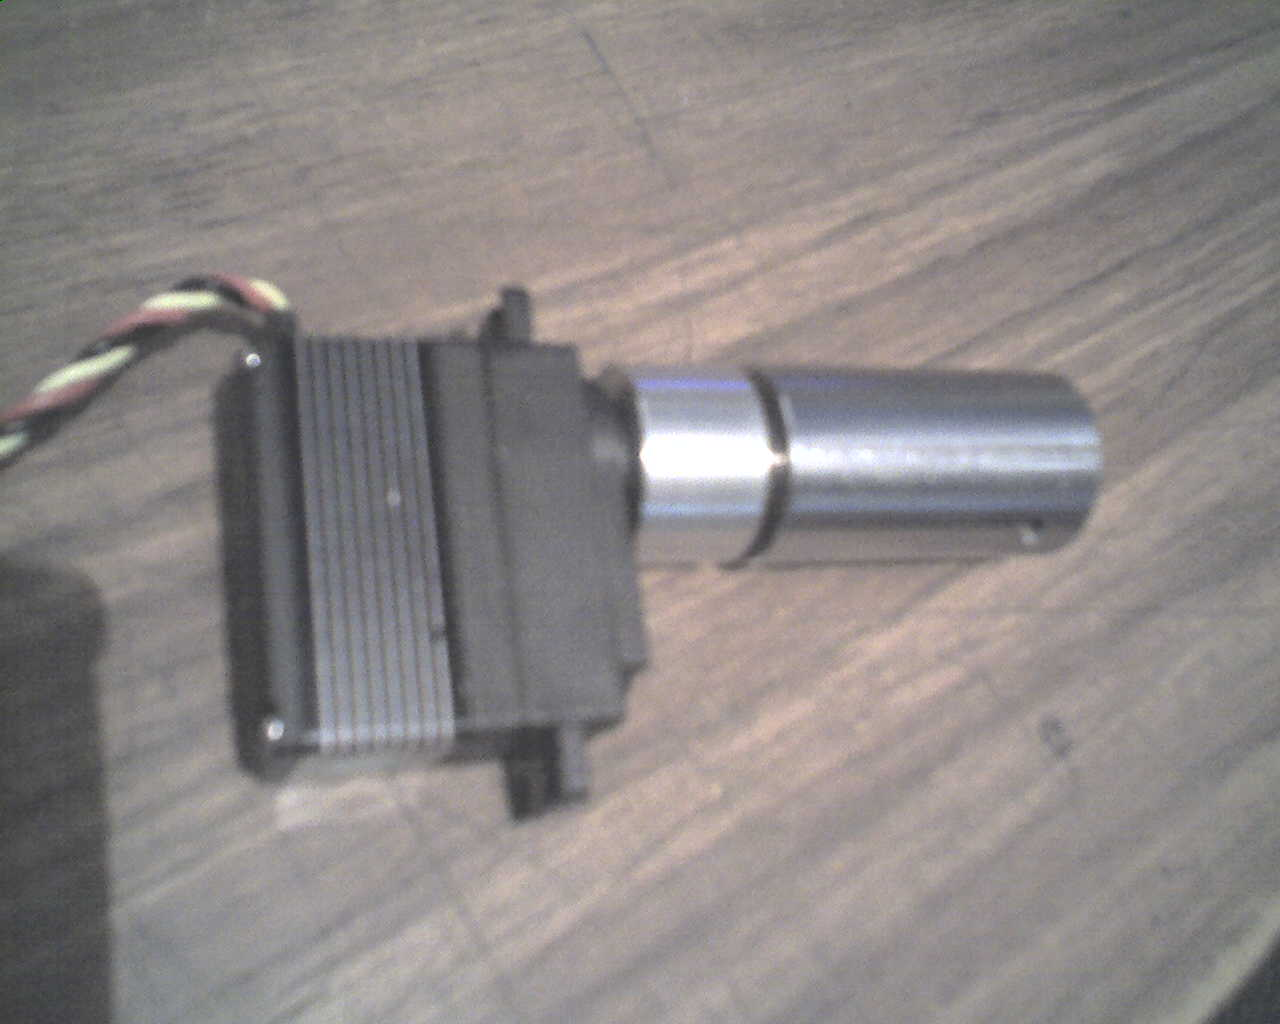
\includegraphics[scale=0.25]{figs/img106.jpg}}
		\caption{Ejes coordenados.}
	\label{fig:DH}
\end{figure}

\begin{table}[h]
	\centering
		\begin{tabular}{|c|c|c|c|c|}
		\hline
			$Eslabon_{i}$	&	$a_{i}$	&	$d_{i}$	&	$\alpha_{i}$ & $\theta_{i}$	\\
			\hline
			0	&	0	&	0	&	0	&	0	\\
			\hline
			1&a1&0&90&q1\\
			\hline
			2&a2&0&0&q2\\
			\hline
			3&a2&0&0&q3\\
			\hline
			4&a1&0&90&q4\\
			\hline
			5&0&0&0&q5\\
			\hline
		\end{tabular}
	\caption{Par�metros de D-H.}
	\label{tab:DH}
\end{table}

Las matrices de transformaci�n Homog�neas obtenidas para cada uno de los eslabones son:\\

\begin{center}

$T_0^1 $= 	\begin{math}
				\left[
				\begin{array}{cccc}
			   	cos(q_1)&               0&         sin(q_1)& 62.82cos(q_1)\\
         sin(q_1)&               0&         cos(q_1)& 62.82sin(q_1)\\
               0&               1&               0&            0 \\
               0&               0&               0&            1

				\end{array}
				\right]
				\end{math}\\
				
\vspace{1cm}

$T_1^2 $= 	\begin{math}
				\left[
				\begin{array}{cccc}
			   	cos(q_2)&	  		 -sin(q_2)&								0&			68.29cos(q_2)\\
          sin(q_2)&          cos(q_2)&                0& 		 68.29sin(q_2)\\
                0&                0&                1&                0\\
                0&                0&                0&                1
				\end{array}
				\right]
				\end{math}\\

\vspace{1cm}				

$T_2^3 $= 	\begin{math}
				\left[
				\begin{array}{cccc}
			   	cos(q_3)&	  		 -sin(q_3)&								0&			68.29cos(q_3)\\
          sin(q_3)&          cos(q_3)&                0& 		 68.29sin(q_3)\\
                0&                0&                1&                0\\
                0&                0&                0&                1

				\end{array}
				\right]
				\end{math}\\
				
\vspace{1cm}				

$T_3^4 $= 	\begin{math}
				\left[
				\begin{array}{cccc}
			   	cos(q_4)&               0&         sin(q_4)& 62.82cos(q_4)\\
         sin(q_4)&               0&         cos(q_4)& 62.82sin(q_4)\\
               0&               1&               0&            0 \\
               0&               0&               0&            1

				\end{array}
				\right]
				\end{math}\\			

\vspace{1cm}

$T_4^5 $= 	\begin{math}
				\left[
				\begin{array}{cccc}
			   	cos(q_5)&	  		 -sin(q_5)&								0&			0)\\
          sin(q_5)&          cos(q_5)&                0& 		 0\\
                0&                0&                1&      0\\
                0&                0&                0&      1

				\end{array}
				\right]
				\end{math}\\
				
				\newpage
				
			
			
{\footnotesize
\begin{center}
				$T_0^5 $= 	
	\begin{math}
\left[
		\begin{array}{ccc}
		\left(\begin{array}{c}
		 cos(q_1)cos(q_5)cos(q_2+q_3+q_4)\\
			   +sin(q_1)sin(q_5)
			   \end{array}\right)&\left(\begin{array}{c}
			   -cos(q_1)sin(q_5)cos(q_2+q_3+q_4)\\
			   +sin(q_1)cos(q_5)
			   \end{array}\right)&cos(q_1)sin(q_2+q_3+q_4\\
			   && \\
\left(\begin{array}{c}
sin(q_1)cos(q_5)cos(q_2+q_3+q_4)\\
-sin(q_1)sin(q_5) \end{array}\right)&\left(\begin{array}{c}
-sin(q_1)sin(q_5)cos(q_2+q_3+q_4)\\
-cos(q_1)cos(q_5)\end{array}\right)&-sin(q_1)sin(q_2+q_3+q_4)\\
   && \\
cos(q_5)sin(q_2+q_3+q_4)&-sin(q_5)sin(q_2+q_3+q_4)&-cos(q_2+q_3+q_4)\\
 & & \\
0&0&0
		\end{array}
				\right]
				\end{math}\\
\end{center}
}
\end{center}

Con este modelo matem�tico es posible generar trayectorias y as� analizar la etapa de caminado. Tambi�n es posible realizar un control de movimiento, sin embargo, este control no ofrecer� la mejor soluci�n, ya que al resolver el problema cinem�tico, no se est�n considerando algunos factores que podr�an afectar al modelo, es por eso que se decide realizar tambi�n un modelado din�mico del sistema.
